%%
%% Beginning of file 'sample62.tex'
%%
%% Modified 2018 January
%%
%% This is a sample manuscript marked up using the
%% AASTeX v6.2 LaTeX 2e macros.
%%
%% AASTeX is now based on Alexey Vikhlinin's emulateapj.cls 
%% (Copyright 2000-2015).  See the classfile for details.

%% AASTeX requires revtex4-1.cls (http://publish.aps.org/revtex4/) and
%% other external packages (latexsym, graphicx, amssymb, longtable, and epsf).
%% All of these external packages should already be present in the modern TeX 
%% distributions.  If not they can also be obtained at www.ctan.org.

%% The first piece of markup in an AASTeX v6.x document is the \documentclass
%% command. LaTeX will ignore any data that comes before this command. The 
%% documentclass can take an optional argument to modify the output style.
%% The command below calls the preprint style  which will produce a tightly 
%% typeset, one-column, single-spaced document.  It is the default and thus
%% does not need to be explicitly stated.
%%
%%
%% using aastex version 6.2
\documentclass[twocolumn]{aastex62}
\usepackage{amsmath}
\usepackage{microtype}
\usepackage{bm}
\usepackage{dsfont}
\usepackage{listings}
\usepackage{url}
\lstset{
	basicstyle=\ttfamily,
	mathescape
}
%% The default is a single spaced, 10 point font, single spaced article.
%% There are 5 other style options available via an optional argument. They
%% can be envoked like this:
%%
%% \documentclass[argument]{aastex62}
%% 
%% where the layout options are:
%%
%%  twocolumn   : two text columns, 10 point font, single spaced article.
%%                This is the most compact and represent the final published
%%                derived PDF copy of the accepted manuscript from the publisher
%%  manuscript  : one text column, 12 point font, double spaced article.
%%  preprint    : one text column, 12 point font, single spaced article.  
%%  preprint2   : two text columns, 12 point font, single spaced article.
%%  modern      : a stylish, single text column, 12 point font, article with
%% 		  wider left and right margins. This uses the Daniel
%% 		  Foreman-Mackey and David Hogg design.
%%  RNAAS       : Preferred style for Research Notes which are by design 
%%                lacking an abstract and brief. DO NOT use \begin{abstract}
%%                and \end{abstract} with this style.
%%
%% Note that you can submit to the AAS Journals in any of these 6 styles.
%%
%% There are other optional arguments one can envoke to allow other stylistic
%% actions. The available options are:
%%
%%  astrosymb    : Loads Astrosymb font and define \astrocommands. 
%%  tighten      : Makes baselineskip slightly smaller, only works with 
%%                 the twocolumn substyle.
%%  times        : uses times font instead of the default
%%  linenumbers  : turn on lineno package.
%%  trackchanges : required to see the revision mark up and print its output
%%  longauthor   : Do not use the more compressed footnote style (default) for 
%%                 the author/collaboration/affiliations. Instead print all
%%                 affiliation information after each name. Creates a much
%%                 long author list but may be desirable for short author papers
%%
%% these can be used in any combination, e.g.
%%
%% \documentclass[twocolumn,linenumbers,trackchanges]{aastex62}
%%
%% AASTeX v6.* now includes \hyperref support. While we have built in specific
%% defaults into the classfile you can manually override them with the
%% \hypersetup command. For example,
%%
%%\hypersetup{linkcolor=red,citecolor=green,filecolor=cyan,urlcolor=magenta}
%%
%% will change the color of the internal links to red, the links to the
%% bibliography to green, the file links to cyan, and the external links to
%% magenta. Additional information on \hyperref options can be found here:
%% https://www.tug.org/applications/hyperref/manual.html#x1-40003
%%
%% If you want to create your own macros, you can do so
%% using \newcommand. Your macros should appear before
%% the \begin{document} command.
%%
\newcommand{\vdag}{(v)^\dagger}
\newcommand\aastex{AAS\TeX}
\newcommand\latex{La\TeX}
\newcommand{\thickbar}[1]{\mathbf{\bar{\text{$#1$}}}}
%% Tells LaTeX to search for image files in the 
%% current directory as well as in the figures/ folder.
\graphicspath{{./}{figures/}}

%% Reintroduced the \received and \accepted commands from AASTeX v5.2
%\received{January 1, 2018}
%\revised{January 7, 2018}
%\accepted{\today}
%% Command to document which AAS Journal the manuscript was submitted to.
%% Adds "Submitted to " the arguement.
%\submitjournal{ApJ}

%% Mark up commands to limit the number of authors on the front page.
%% Note that in AASTeX v6.2 a \collaboration call (see below) counts as
%% an author in this case.
%
%\AuthorCollaborationLimit=3
%
%% Will only show Schwarz, Muench and "the AAS Journals Data Scientist 
%% collaboration" on the front page of this example manuscript.
%%
%% Note that all of the author will be shown in the published article.
%% This feature is meant to be used prior to acceptance to make the
%% front end of a long author article more manageable. Please do not use
%% this functionality for manuscripts with less than 20 authors. Conversely,
%% please do use this when the number of authors exceeds 40.
%%
%% Use \allauthors at the manuscript end to show the full author list.
%% This command should only be used with \AuthorCollaborationLimit is used.

%% The following command can be used to set the latex table counters.  It
%% is needed in this document because it uses a mix of latex tabular and
%% AASTeX deluxetables.  In general it should not be needed.
%\setcounter{table}{1}

%%%%%%%%%%%%%%%%%%%%%%%%%%%%%%%%%%%%%%%%%%%%%%%%%%%%%%%%%%%%%%%%%%%%%%%%%%%%%%%%
%%
%% The following section outlines numerous optional output that
%% can be displayed in the front matter or as running meta-data.
%%
%% If you wish, you may supply running head information, although
%% this information may be modified by the editorial offices.
\shorttitle{DRAFT 1}
\shortauthors{DRAFT 1}
%%
%% You can add a light gray and diagonal water-mark to the first page 
%% with this command:
% \watermark{text}
%% where "text", e.g. DRAFT, is the text to appear.  If the text is 
%% long you can control the water-mark size with:
%  \setwatermarkfontsize{dimension}
%% where dimension is any recognized LaTeX dimension, e.g. pt, in, etc.
%%
%%%%%%%%%%%%%%%%%%%%%%%%%%%%%%%%%%%%%%%%%%%%%%%%%%%%%%%%%%%%%%%%%%%%%%%%%%%%%%%%

%% This is the end of the preamble.  Indicate the beginning of the
%% manuscript itself with \begin{document}.

\begin{document}

\title{DRAFT 1 Processing JUPITER Hydrodynamics Simulation Data for Visualisation in Paraview DRAFT 1}

%% LaTeX will automatically break titles if they run longer than
%% one line. However, you may use \\ to force a line break if
%% you desire. In v6.2 you can include a footnote in the title.

%% A significant change from earlier AASTEX versions is in the structure for 
%% calling author and affilations. The change was necessary to implement 
%% autoindexing of affilations which prior was a manual process that could 
%% easily be tedious in large author manuscripts.
%%
%% The \author command is the same as before except it now takes an optional
%% arguement which is the 16 digit ORCID. The syntax is:
%% \author[xxxx-xxxx-xxxx-xxxx]{Author Name}
%%
%% This will hyperlink the author name to the author's ORCID page. Note that
%% during compilation, LaTeX will do some limited checking of the format of
%% the ID to make sure it is valid.
%%
%% Use \affiliation for affiliation information. The old \affil is now aliased
%% to \affiliation. AASTeX v6.2 will automatically index these in the header.
%% When a duplicate is found its index will be the same as its previous entry.
%%
%% Note that \altaffilmark and \altaffiltext have been removed and thus 
%% can not be used to document secondary affiliations. If they are used latex
%% will issue a specific error message and quit. Please use multiple 
%% \affiliation calls for to document more than one affiliation.
%%
%% The new \altaffiliation can be used to indicate some secondary information
%% such as fellowships. This command produces a non-numeric footnote that is
%% set away from the numeric \affiliation footnotes.  NOTE that if an
%% \altaffiliation command is used it must come BEFORE the \affiliation call,
%% right after the \author command, in order to place the footnotes in
%% the proper location.
%%
%% Use \email to set provide email addresses. Each \email will appear on its
%% own line so you can put multiple email address in one \email call. A new
%% \correspondingauthor command is available in V6.2 to identify the
%% corresponding author of the manuscript. It is the author's responsibility
%% to make sure this name is also in the author list.
%%
%% While authors can be grouped inside the same \author and \affiliation
%% commands it is better to have a single author for each. This allows for
%% one to exploit all the new benefits and should make book-keeping easier.
%%
%% If done correctly the peer review system will be able to
%% automatically put the author and affiliation information from the manuscript
%% and save the corresponding author the trouble of entering it by hand.

\correspondingauthor{Evert Nasedkin}
\email{evertn@student.ethz.ch}

\author{Evert Nasedkin}
\affil{ETH Zurich}

%% Note that the \and command from previous versions of AASTeX is now
%% depreciated in this version as it is no longer necessary. AASTeX 
%% automatically takes care of all commas and "and"s between authors names.

%% AASTeX 6.2 has the new \collaboration and \nocollaboration commands to
%% provide the collaboration status of a group of authors. These commands 
%% can be used either before or after the list of corresponding authors. The
%% argument for \collaboration is the collaboration identifier. Authors are
%% encouraged to surround collaboration identifiers with ()s. The 
%% \nocollaboration command takes no argument and exists to indicate that
%% the nearby authors are not part of surrounding collaborations.

%% Mark off the abstract in the ``abstract'' environment. 
\begin{abstract}
\end{abstract}

%% Keywords should appear after the \end{abstract} command. 
%% See the online documentation for the full list of available subject
%% keywords and the rules for their use.
\keywords{}

%% From the front matter, we move on to the body of the paper.
%% Sections are demarcated by \section and \subsection, respectively.
%% Observe the use of the LaTeX \label
%% command after the \subsection to give a symbolic KEY to the
%% subsection for cross-referencing in a \ref command.
%% You can use LaTeX's \ref and \label commands to keep track of
%% cross-references to sections, equations, tables, and figures.
%% That way, if you change the order of any elements, LaTeX will
%% automatically renumber them.
%%
%% We recommend that authors also use the natbib \citep
%% and \citet commands to identify citations.  The citations are
%% tied to the reference list via symbolic KEYs. The KEY corresponds
%% to the KEY in the \bibitem in the reference list below. 

\section{Introduction} \label{sec:intro}
This report examines the software developed to process JUPITER hydrodynamic simulation data to allow for visualisation using the open source program Paraview.

\subsection{JUPITER}\label{sec:jup}
JUPITER is a 3D, nested mesh simulation program that solves the hydrodynamic and radiative transfer equations using a high order Godunov scheme. This allows a spatial resolution of about 0.8 Jupiter radii at the finest mesh level. 
The radiative transfer is calculated with the method of Commer\c{c}on et al. (2011), with Dirichlet boundary conditions on the boundaries between mesh levels.
Thus JUPITER solves for mass and momentum conservation, along with total energy, accounting for coupling between thermal  radiative energy ($\epsilon_{rad}$). The governing equations for the program are therefore:
\begin{align}\label{eqns:hydro}
&\frac{\partial\rho}{\partial t} + \nabla \cdot \left(\rho\mathbf{v}\right) = 0\\
&\frac{\partial\left(\rho\mathbf{v}\right)}{\partial t} + \nabla \cdot \left(\rho\mathbf{v} \otimes \mathbf{v}\right) + \nabla P = -\rho\mathbf{v}\cdot\nabla\Phi + \nabla \cdot \bm{\bar{\tau}}\\
\begin{split}
&\frac{\partial E}{\partial t} + \nabla\cdot\left[\left(P \mathds{1}- \bm{\bar{\tau}} \right) \cdot \mathbf{v} + E\mathbf{v}\right] = \\&\qquad\qquad\qquad\quad\rho \mathbf{v}\cdot\nabla\Phi - \rho\kappa_{P}c\left(\frac{B\left(T\right)}{c} - \epsilon_{rad}\right)
\end{split}\\
&\frac{\partial \epsilon_{rad}}{\partial t} = -\nabla \cdot F_{rad} + \rho\kappa_{P}c\left(\frac{B\left(T\right)}{c} - \epsilon_{rad}\right)
\end{align}

The density is given by $\rho$, E is the total gas energy (U + K), $\mathbf{v}$ is the gas velocity, $P$ is pressure, $\Phi$ is the gravitational potential and $T$ is temperature. $\kappa_{P}$ is the Planck opacity from eqn. \ref{eqn:kp} and $B(T)$ is the thermal blackbody radiation power, given by $4\sigma T^{4}$. $c$ is the speed of light and $\sigma$ is the Stephan-Boltzmann constant. $\mathds{1}$ is the identity and $\bm{\bar{\tau}}$ is the stress tensor:
\begin{equation}
\bm{\bar{\tau}} = 2\rho\nu\left(\bm{\bar{D}} - \frac{1}{3}\left(\nabla\cdot\mathbf{v}\right)\mathds{1}\right)
\end{equation}

The Planck Opacity is defined as 
\begin{equation}\label{eqn:kp}
\kappa_{P} = \frac{\int_{0}^{\infty}\kappa_{\nu}B_{\nu}\left(T\right)d\nu}{\int_{0}^{\infty}B_{\nu}\left(T\right)d\nu}
\end{equation}
where $\nu$ is the kinematic velocity and $\mathds{\bar{D}}$ is the strain tensor. Finally $F_{rad}$ is given by:
\begin{equation}
F_{rad} = -\frac{c\lambda}{\rho\kappa_{R}}\nabla\epsilon_{rad}
\end{equation}
$\kappa_{R}$ is the Rosseland mean opacity, and $\lambda$ is a flux limiter to smooth the transition between optically thick and thin regions.

The equation of state of the system is taken to be 
\begin{equation}
P = \left(\gamma - 1\right)\epsilon
\end{equation}
where $\epsilon = \rho c_{v}T$ and the adiabatic index $\gamma = 1.43$.

JUPITER can then be supplied with a given set of initial conditions and system properties, and will calculate each of the hydrodynamic fields at each time step to explore planet-disk interactions and related physics.
\subsection{Adaptive Mesh Refinement}\label{sec:amr}
\textcolor{red}{TALK TO JUDIT TO MAKE SURE THIS SECTION IS CORRECT}

The nested mesh system used in JUPITER is an example of adaptive mesh refinement (AMR) techniques. 
In general, AMR improves computational speed for a given maximum resolution, as it reduces the number of mesh elements in the grid while maintaining the high resolution in the region of interest as seen in fig. \ref{fig:mesh}. 
In JUPITER, the mesh is not truly adaptive, as the refinement regions are predefined in the region of the planet embedded in the circumstellar disk.
Other AMR techniques could refine the mesh only in regions of steep density or velocity gradients. 
However, as circumstellar are not a static-flow environment, the location of these gradients changes over time, and it would be difficult to manage a constantly changing grid. 
In contrast, JUPITER uses a static grid, and allows the flow to evolve throughout the grid over time.

Boundary conditions must be defined for each of the mesh regions, and this is achieved by interpolating the results of a coarse mesh to provide the boundary conditions for the next level. 
The results of the fine level are then used to improve the results of the coarse mesh in the region. 
This is iterated for each mesh refinement level, with the edge length in each dimension being half that of the previous, coarser level. 
\begin{figure}[h]
	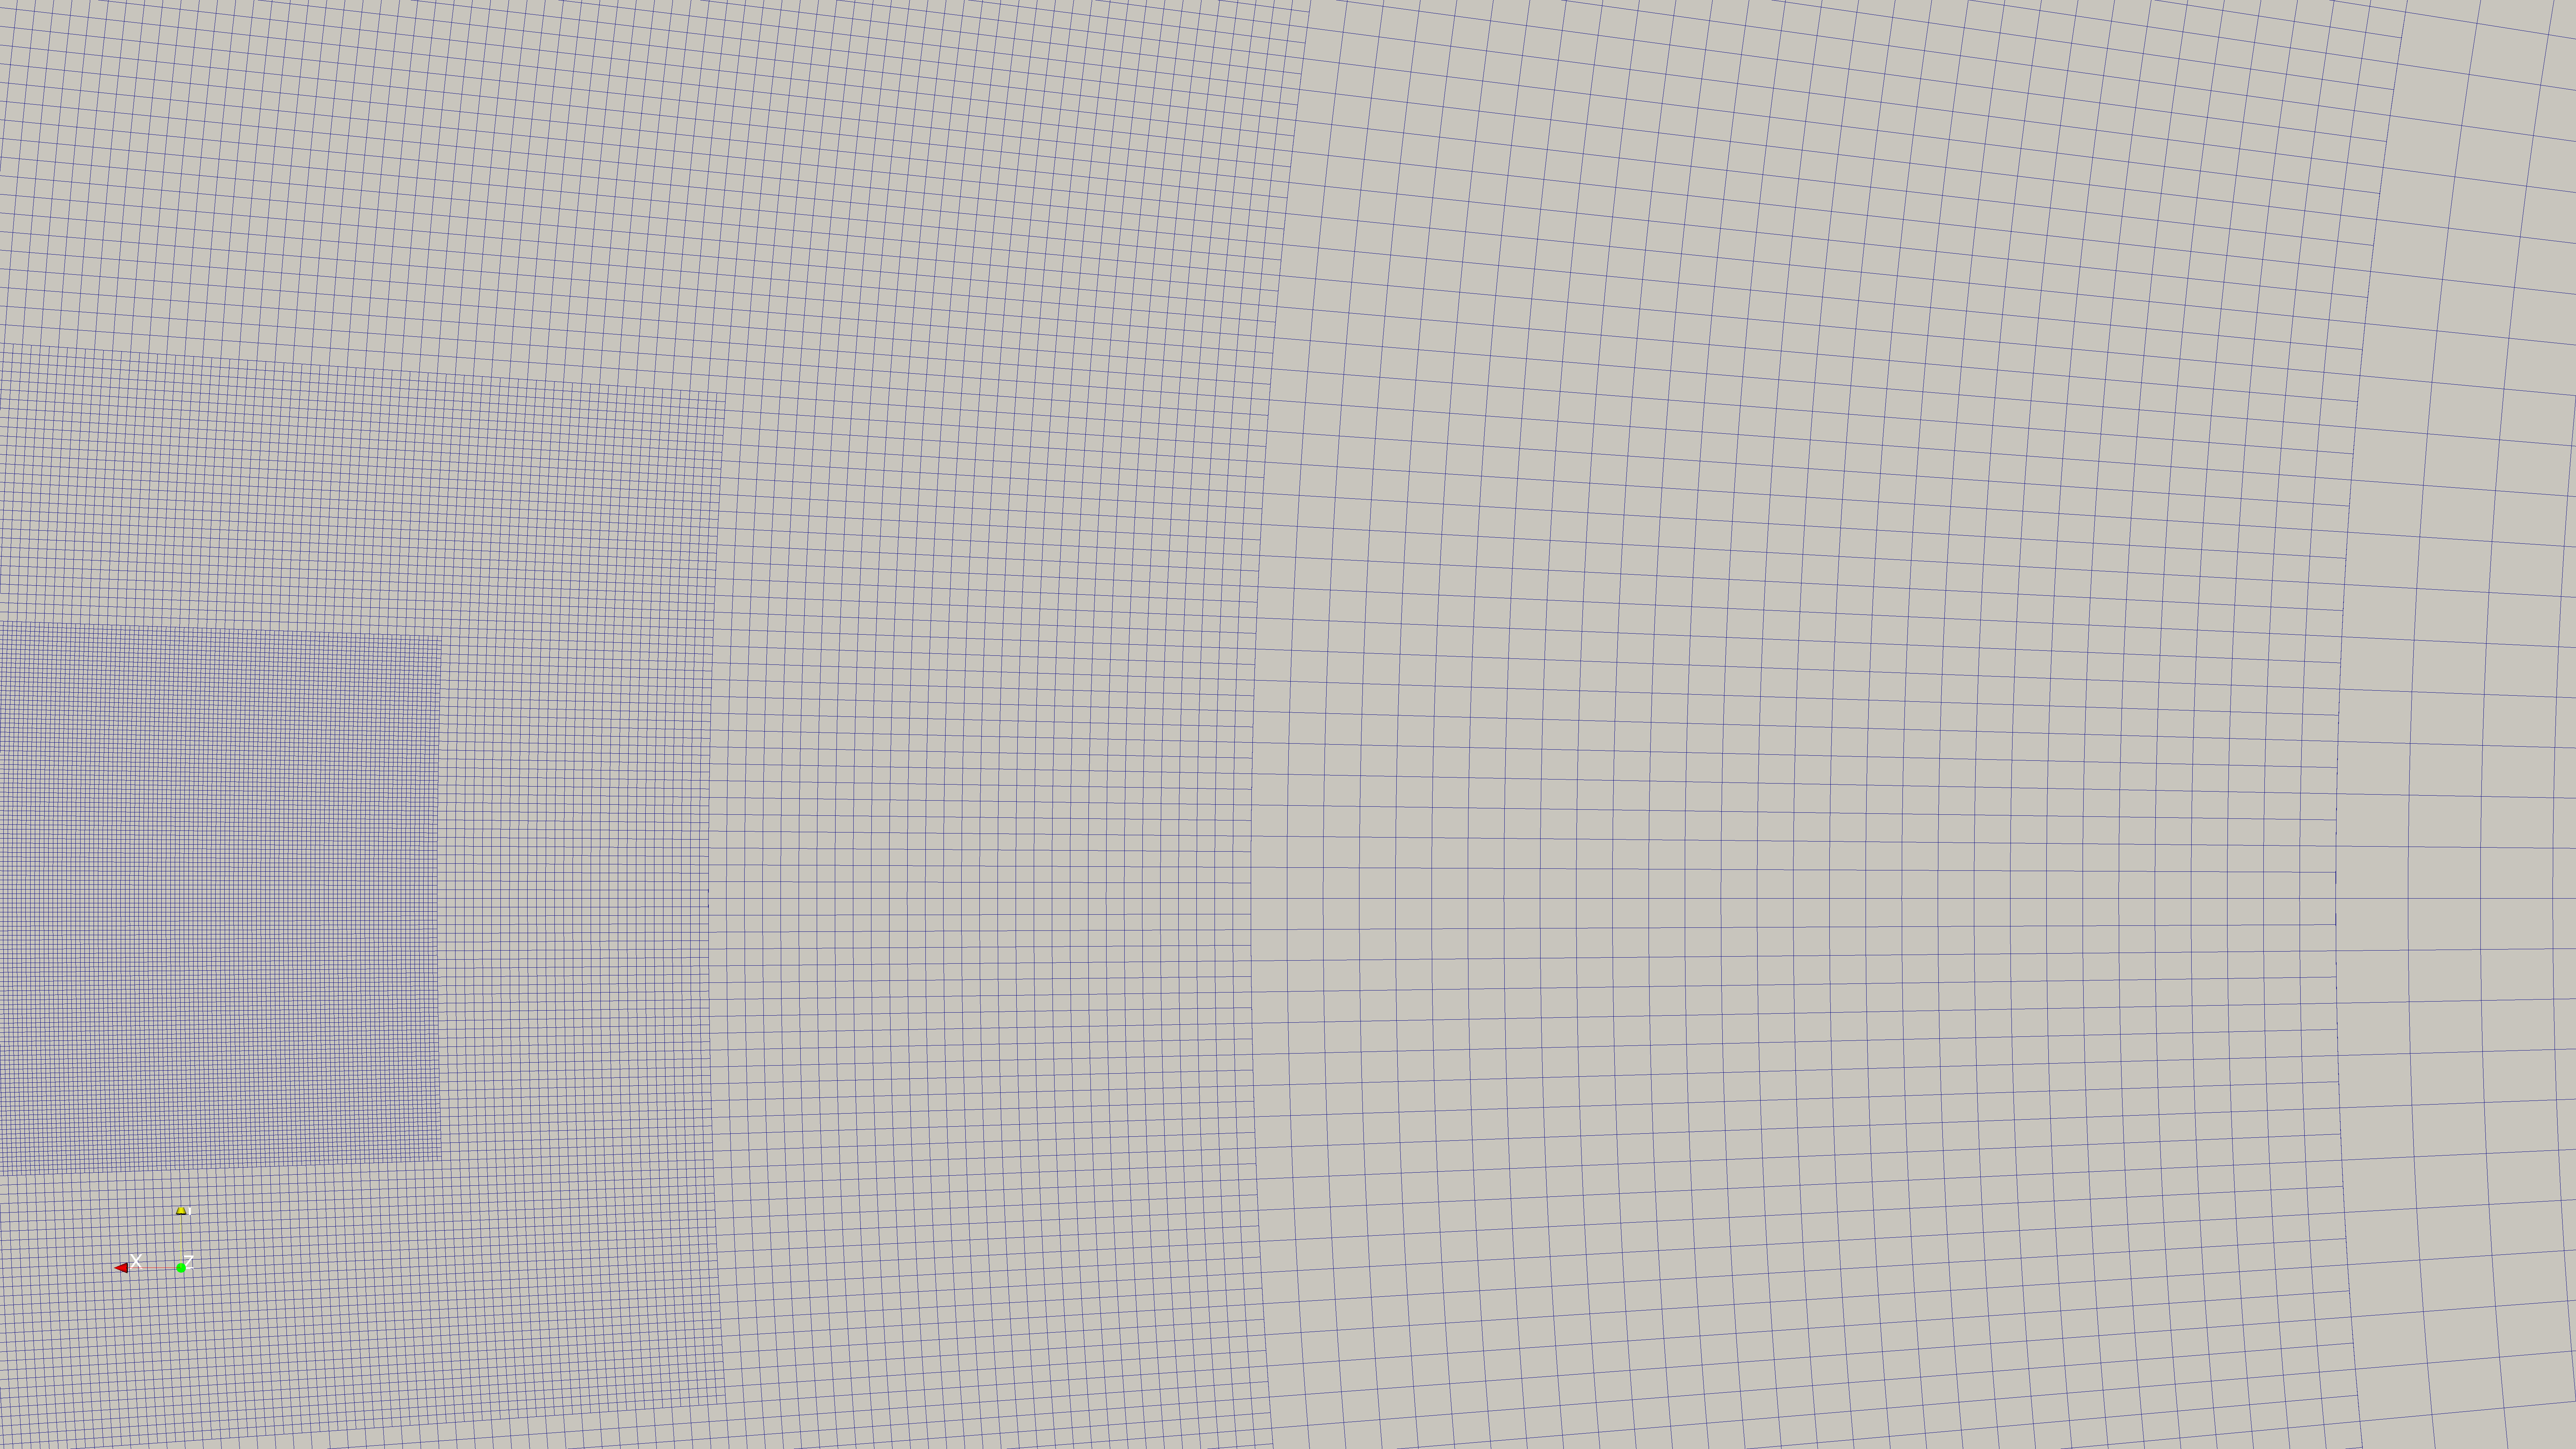
\includegraphics[width=\linewidth]{figures/meshface.png}
	\caption{\label{fig:mesh}Nested mesh levels around the location of the planet from a JUPITER simulation.}
\end{figure}
\subsection{Outputs}\label{sec:out}
As JUPITER relies on parallel computation, each core will output the hydrodynamic fields in its mesh region. These can be stitched together to create output files for each hydrodynamic field over the whole disk.

The first output file is a descriptor file that provides simulation properties, along with the positions in spherical coordinates of each of the vertices of the mesh for each mesh level. 
For this report $phi$ represents the azimuthal angle, and $theta$ the polar angle from the z-axis, and coordinates are generally ordered ($\phi$, $r$, $\theta$). 
The file is structured as follows:
\textcolor{red}{TALK TO JUDIT ABOUT WHAT ELSE IS IN THE DESCRIPTOR FILE}
\begin{lstlisting}
[line 1]
[line 2]
[line 3]
[line 4]
[line 5]
[line 6]
[N$_{\phi}$ N$_{r}$ N$_{\theta}$]
[line 8]
[$\phi$ axis]
[$r$ axis]
[$\theta$ axis]
\end{lstlisting}
This structure is then repeated sequentially for each mesh refinement level, from coarse to fine. The first and last two components of each axis are ghost cells, and should not be read in. The number of components along each axis (e.g. $N_{\phi}$) takes this accounts for this, however it assumes zero index counting. Thus if there are 681 $\phi$ components, the descriptor file will read 680, and the total axis in the file will contain 685 elements.

Each hydrodynamic field is stored in a data file, with a data point for each cell of the mesh. Note that while the descriptor file stores the locations of the vertices of the cells, all of the field data is defined at the barycentre of a given cell. The data is stored as binary doubles, and is ordered such that for a given coordinates ($\phi_{i}$, $r_{j}$, $\theta_{k}$), $i$ is iterated the fastest and $k$ the slowest. For vector data (velocities), each component of the vector is ordered as a scaler, with the azimuthal velocity listed first in its entirety, followed by the radial component, followed by the polar component. This ordering is also user adjustable in JUPITER, and may change. All data is stored in code units, and must be converted to physical units after read in.

Many of these hydrodynamic fields cannot be processed for visualisation with existing software (e.g. RadMC3D), so a conversion tool was necessary to allow for visualisation in Paraview.
\section{Processing Tools}\label{sec:code}
All of the tools described on this section are available on Github: \url{https://github.com/nenasedk/JUPITER_VTKFileConversion}
\subsection{VTK File Structure}\label{sec:vtk}
Paraview uses the VTK file format to store data for visualisation. While a modern xml format exists, the legacy format is simpler to use and has much more extensive documentation, and was thus chosen for this project. Future work could explore the usage of a VTK format developed for adaptive mesh grids.

The legacy VTK format is structured into 5 parts:
\begin{enumerate}
	\item The file version and identifier, which must be exactly \verb|# vtk DataFile Version x.x|
	For this project we are using VTK version 2.0.
	\item The header, one line terminated by \verb|\n| to describe the data.
	\item File format. Either \verb|ascii|$\lvert$\verb|binary|
	\item Dataset structure. This describes the geometry and topology of the dataset, and consists of the word \verb|DATASET| followed by a keyword description of the data. We use an Unstructured Grid to describe the data.
	An unstructured grid requires both a list of coordinates and a list of connections to fully specify the locations and connections of each cell in the grid.
	
	Following the keyword is the list of coordinates used to describe the data. This initiated by line \verb|POINTS n datatype|, where n is the number of coordinates and datatype is a C type (we use doubles). The JUPITER coordinate grid is listed in order $\phi$, $r$, $\theta$, with $\phi$ iterating the fastest and $\theta$ the slowest. Each coordinate vector is converted to a Cartesian grid before being written to file, so the VTK file will contain the x,y,z components of each vertex in the mesh in CGS units, centred on the star. Each mesh level is appended subsequently from coarsest to finest.
	
	After the list of coordinates, the cells are listed. This section begins with the line \verb|CELLS m| where m is the number of cells. Each row begins with the number of vertices of the cell, followed by the index of the coordinates of each vertex of the cell. We use a hexahedral cell type (cell type 8), and a description of the algorithm to compute the indices is found in sec. \ref{sec:code}. 
	
	Following the list of cells is the list of cell types for each cell. This is started by the line \verb|CELL_TYPES m| where m is the number of cells. All of the cells used in JUPITER are hexahedral (type 12).
	\item Dataset attributes. This can be either \verb|POINT_DATA|, where each datapoint is located at a mesh vertex, or \verb|CELL_DATA|, where each datapoint is located at the centre of a cell. All JUPITER hydro fields are \verb|CELL_DATA|. Additionally, each datapoint can be either a \verb|SCALAR| or \verb|VECTOR|, the latter of which is used to store velocities.
\end{enumerate}
An example file is included in Appendix A.
\subsection{Data Processing Methods}\label{sec:code}
\textbf{Requirements}

To run the python conversion script the user must have installed at minimum:
\begin{itemize}
	\item Python 2.7 or greater
	\item numpy package
	\item astropy package
	\item vtk package v8.1.1
\end{itemize}

\textbf{Overview}

To process the outputs of the JUPITER simulations into the VTK fileformat, a python class was written. 
The class has a range of user settable functions, allowing the user to write a script to wrap the class for a given conversion job, or use the interactive command line interface written for the class.
In general, the user must provide the input and output directories, the output number, the number of mesh refinement levels, the hydrodynamic field to convert, the orbital radius of the planet in AU and the mass of the star in solar masses.

The program flow is as follows:
\begin{enumerate}
	\item Setup directories and filenames, and set science variables.
	\item Read in the coordinates from the descriptor file. From the axes read in, build a grid of 3D coordinates ($\phi_{i}$, $r_{j}$, $\theta_{k}$), and create an additional grid with the coordinates converted to Cartesian. 
	\item For each mesh level, define the boundaries of the next finest level. Cells (NOT grid points) within this region of interest (ROI) will be ignored.
	\item Compute the indices of each vertex of each cell. This is achieved using a stride calculation in the \verb|ComputeStructuredCell()| function:	
	\begin{itemize}
		 \item Label the indices from 0 to 7, counter clockwise and from bottom to top. Thus the 'bottom' level of each hexahedral cell consists of indices 0-3, the top from 4-7, with index 4 directly above index 0.
		 \item The axis are iterated $phi$ fastest and $\theta$ slowest. Therefore index 1 will be one greater, but index 3 will be a full $\phi$ axis farther along than index 0. Likewise, index 4 will be an $r-\phi$ plane greater than index 0.
		 \item Iterate through each axis, incrementing the counters. Any cells with one or more vertices within the ROI will be skipped, but their index in the total list of cells is stored.
 	\end{itemize}
	\item Read in the data from the descriptor file, reshaping vector (velocity) data as necessary. Remove the datapoints with the indices of the removed cells.
	\item Write the data to a binary or ascii VTK file. If the output file already exists, the user can choose to overwrite the file, or append new data to the existing file.
\end{enumerate}

\textbf{Usage}

To use the command line interface simply use \verb|python Convert.py|
Within the Convert.py script, the user can change whether to output to a binary or ascii VTK file, as well as the location of the input data from JUPITER. This data must be in a folder labelled output, and the default path to this directory is to use the current working directory.

A second interface has been developed to allow for easier scripting of inputs. To use this, use:
\verb|python script_convert.py [first] [grid level]\ | \newline \verb|[radius] [mass] -l [last] -b [binary/ascii] -d\ |\newline\verb|[dir] [field list]|

Or without all optional tagged arguments:\newline
\verb|python script_convert.py first [grid_level]\ |\newline \verb|[radius] [mass] [field list]|

Tagged arguments can be placed in any order, but the field list must be the last argument passed.
\begin{itemize}
	\item \verb|[first]| The first simulation output to process.
	\item \verb|- l [last]| The last simulation output to process. Assumes that all integers between first and last exist and should be processed.
	\item \verb|[grid_level]| The mesh refinement level.
	\item \verb|[radius]| The orbital radius of the planet in AU.
	\item \verb|[mass]| The mass of the star in solar masses.
	\item \verb|[-b binary/ascii]| A string (b)inary or (a)scii to set the output file type. Binary is recommended.
	\item \verb|[-d dir]| Directory where the output folder from JUPITER is located
	\item \verb|[field_list]| A list of space separated strings denoting which hydro fields should be converted.
\end{itemize}
\section{Results}\label{sec:res}
\begin{figure}
	\centering
	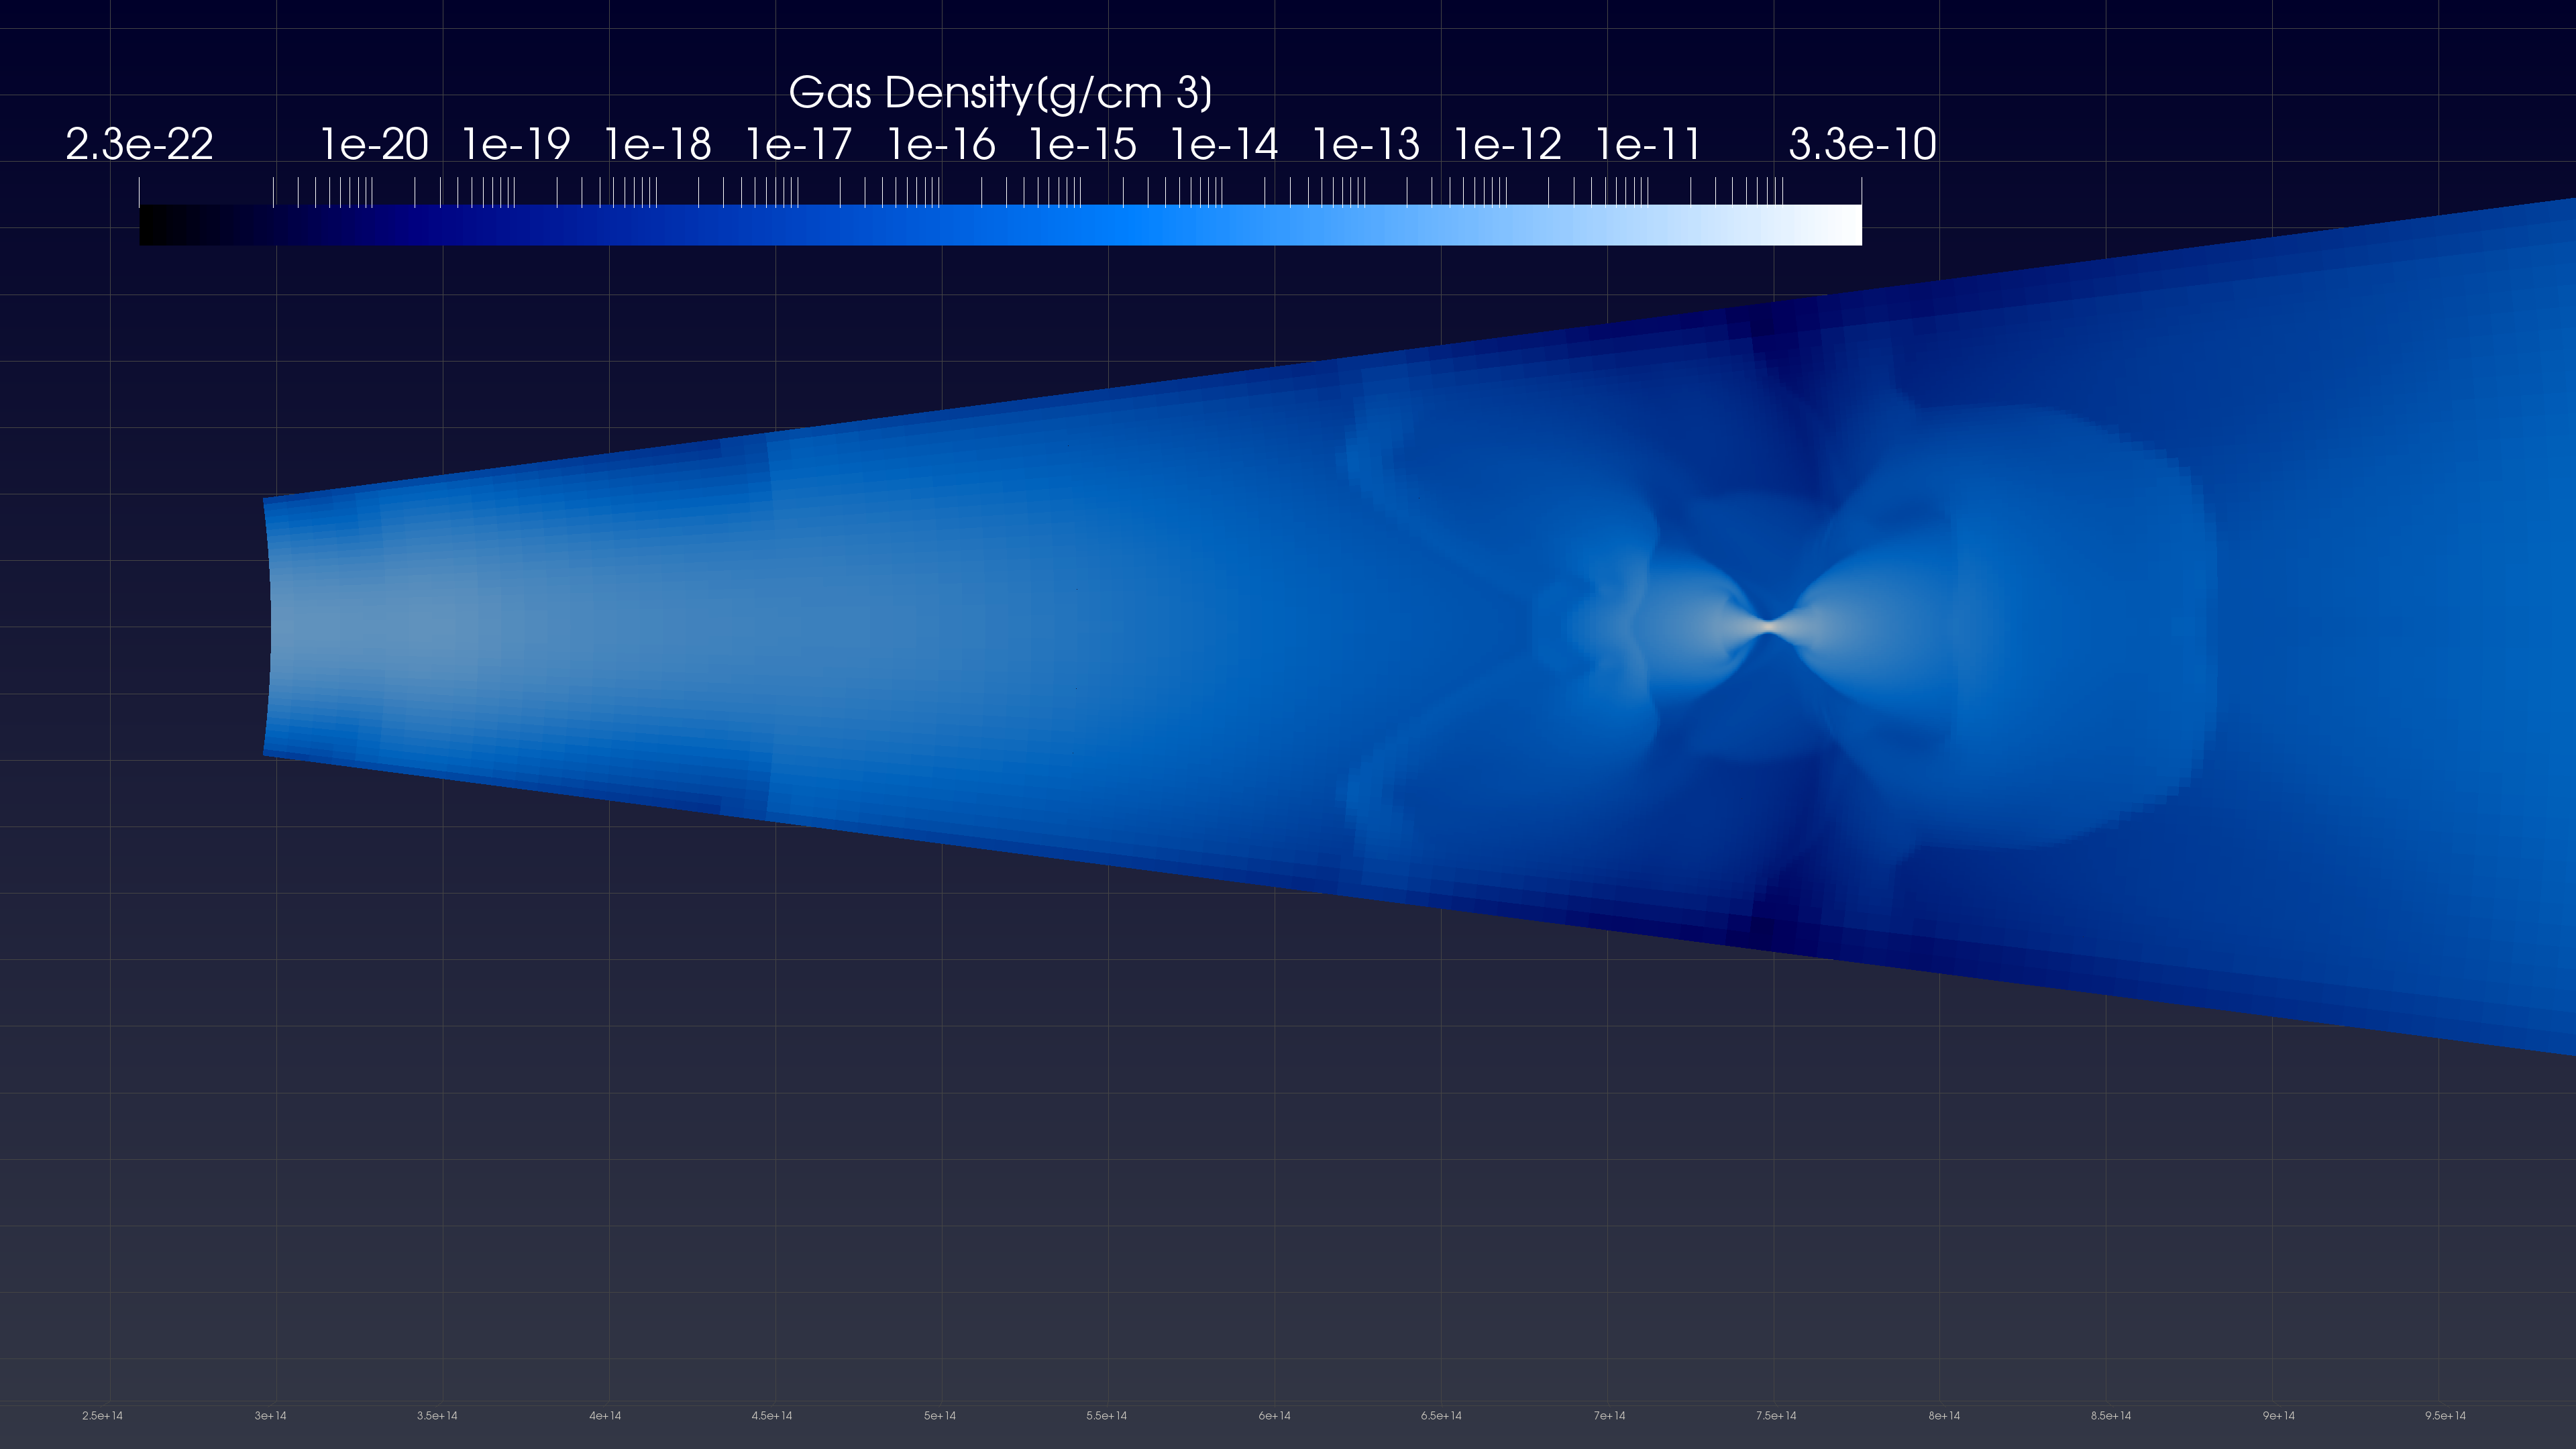
\includegraphics[width=0.9\linewidth]{figures/Dens5YCut0Zoom.png}
	\caption{\label{fig:dens} Cross section of gas density of the circumplanetary disk of a planet embedded at 50 AU in the circumstellar disk of a 1 solar mass star.}
\end{figure}
\begin{figure}
	\centering
	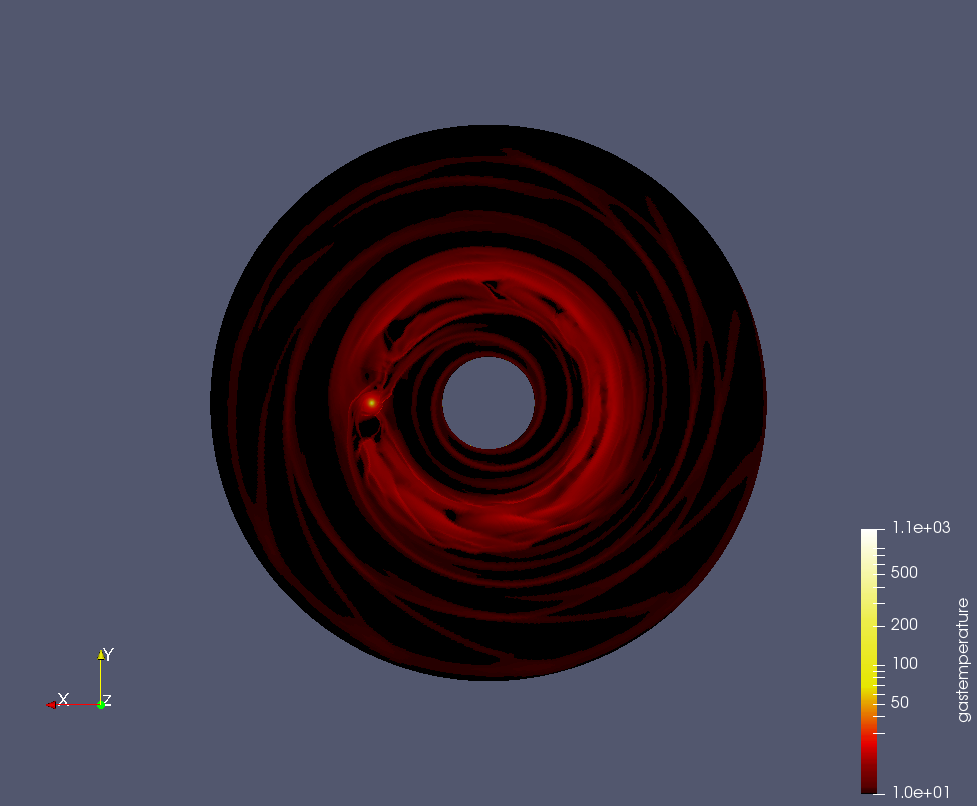
\includegraphics[width=0.9\linewidth]{figures/Temp/GasTempMidplane.png}
	\caption{\label{fig:temp} Temperature of the midplane of the circumstellar disk.}
\end{figure}
\section{Conclusions}\label{sec:con}
\section{Acknowledgements}


%% The reference list follows the main body and any appendices.
%% Use LaTeX's thebibliography environment to mark up your reference list.
%% Note \begin{thebibliography} is followed by an empty set of
%% curly braces.  If you forget this, LaTeX will generate the error
%% "Perhaps a missing \item?".
%%
%% thebibliography produces citations in the text using \bibitem-\cite
%% cross-referencing. Each reference is preceded by a
%% \bibitem command that defines in curly braces the KEY that corresponds
%% to the KEY in the \cite commands (see the first section above).
%% Make sure that you provide a unique KEY for every \bibitem or else the
%% paper will not LaTeX. The square brackets should contain
%% the citation text that LaTeX will insert in
%% place of the \cite commands.

%% We have used macros to produce journal name abbreviations.
%% \aastex provides a number of these for the more frequently-cited journals.
%% See the Author Guide for a list of them.

%% Note that the style of the \bibitem labels (in []) is slightly
%% different from previous examples.  The natbib system solves a host
%% of citation expression problems, but it is necessary to clearly
%% delimit the year from the author name used in the citation.
%% See the natbib documentation for more details and options.

\begin{thebibliography}{}

\bibitem[Astropy Collaboration et al.(2013)]{2013A&A...558A..33A} Astropy Collaboration, Robitaille, T.~P., Tollerud, E.~J., et al.\ 2013, \aap, 558, A33 
\bibitem[Bertin \& Arnouts(1996)]{1996A&AS..117..393B} Bertin, E., \& Arnouts, S.\ 1996, \aaps, 117, 393 
\bibitem[Corrales(2015)]{2015ApJ...805...23C} Corrales, L.\ 2015, \apj, 805, 23
\bibitem[Ferland et al.(2013)]{2013RMxAA..49..137F} Ferland, G.~J., Porter, R.~L., van Hoof, P.~A.~M., et al.\ 2013, \rmxaa, 49, 137
\bibitem[Hanisch \& Biemesderfer(1989)]{1989BAAS...21..780H} Hanisch, R.~J., \& Biemesderfer, C.~D.\ 1989, \baas, 21, 780 
\bibitem[Lamport(1994)]{lamport94} Lamport, L. 1994, LaTeX: A Document Preparation System, 2nd Edition (Boston, Addison-Wesley Professional)
\bibitem[Schwarz et al.(2011)]{2011ApJS..197...31S} Schwarz, G.~J., Ness, J.-U., Osborne, J.~P., et al.\ 2011, \apjs, 197, 31  
\bibitem[Vogt et al.(2014)]{2014ApJ...793..127V} Vogt, F.~P.~A., Dopita, M.~A., Kewley, L.~J., et al.\ 2014, \apj, 793, 127  
%Szul´agyi,\ J., PhD thesis: “Gas accretion onto Jupitermass
%Planets”, 2015, https://people.phys.ethz.ch/ judits/thesisszulagyi.pdf
\end{thebibliography}
\newpage


\section*{Appendix A}
An example of a simple VTK file:
\begin{lstlisting}
# vtk DataFile Version 2.0
Jupiter Simulation Data
ASCII
DATASET UNSTRUCTURED_GRID
POINTS n double
p$_{0x}$ p$_{0y}$ p$_{0z}$
...
p$_{(n-1)x}$ p$_{(n-1)y}$ p$_{(n-1)z}$

CELLS m 
nVert$_{0}$ i0 i1 i2 ... i()nVert$_{0}$-1)
...
nVert$_{(m-1)}$ i0 i1 i2 ... i(nVert$_{(m-1)}$-1)

CELL_TYPE m 
type$_{0}$
..
type$_{(m-1)}$

CELL_DATA m
SCALARS name double
LOOKUP_TABLE default
s$_{0}$
...
s$_{(m-1)}$
\end{lstlisting}

%% This command is needed to show the entire author+affilation list when
%% the collaboration and author truncation commands are used.  It has to
%% go at the end of the manuscript.
%\allauthors

%% Include this line if you are using the \added, \replaced, \deleted
%% commands to see a summary list of all changes at the end of the article.
%\listofchanges

\end{document}

% End of file `sample62.tex'.
